%!TEX root=../../main.tex

\section{Exercises}

% Chapter 8 exercises
% 
% many problems drawn from OI 4 source files
%__________________
\subsection{Inference for a single proportion}

% current commented numbers are from oi4, and our sequence oibio

% oibio 1
% oi4 1

\eoce{\qt{Vegetarian college students\label{veg_coll_students_CLT}} Suppose that 8\% 
of college students are vegetarians. Determine if the following statements are 
true or false, and explain your reasoning.
\begin{parts}
\item The distribution of the sample proportions of vegetarians in random 
samples of size 60 is approximately normal since $n \ge 30$. 
\item The distribution of the sample proportions of vegetarian college 
students in random samples of size 50 is right skewed.
\item A random sample of 125 college students where 12\% are vegetarians 
would be considered unusual. 
\item A random sample of 250 college students where 12\% are vegetarians 
would be considered unusual.
\item The standard error would be reduced by one-half if we increased the 
sample size from 125 to~250.
\end{parts}
 
}{}

% oibio 2
% oi4 2

\eoce{\qt{Young Americans, Part I\label{young_americans_CLT_1}} About 77\% of 
young adults think they can achieve the American dream. Determine if the 
following statements are true or false, and explain your reasoning.
\footfullcite{news:youngAmericans1}
\begin{parts}
\item The distribution of sample proportions of young Americans who think 
they can achieve the American dream in samples of size 20 is left skewed.
\item The distribution of sample proportions of young Americans who think 
they can achieve the American dream in random samples of size 40 is 
approximately normal since $n \ge 30$. 
\item A random sample of 60 young Americans where 85\% think they can achieve 
the American dream would be considered unusual.
\item A random sample of 120 young Americans where 85\% think they can 
achieve the American dream would be considered unusual.
\end{parts}
}{}

% oibio 3
% oi4 5

\eoce{\qt{Gender equality\label{gender_equality}}
The General Social Survey asked a random sample of
1,390 Americans the following question:
``On the whole, do you think it should or should not be
the government's responsibility to  promote equality
between men and women?''
82\% of the respondents said it ``should be''.
At a 95\% confidence level, this sample has 2\% margin of error.
Based on this information, determine if the following statements
are true or false, and explain your reasoning.\footfullcite{data:gss}
\begin{parts}
\item We are 95\% confident that between 80\% and 84\% of Americans in this 
sample think it's the government's responsibility to promote equality between 
men and women.
\item We are 95\% confident that between 80\% and 84\% of all Americans 
think it's the government's responsibility to promote equality between 
men and women.
\item If we considered many random samples of 1,390 Americans, and we calculated 
95\% confidence intervals for each, 95\% of these intervals would include the 
true population proportion of Americans who think it's the government's 
responsibility to promote equality between men and women.
\item In order to decrease the margin of error to 1\%, we would need to 
quadruple (multiply by 4) the sample size.
\item Based on this confidence interval, there is sufficient evidence to 
conclude that a majority of Americans think it's the government's responsibility 
to promote equality between men and women.
\end{parts}

% n = 1390
% should be: 1142
% p = 1142/1390 = 0.82
% me = sqrt(.82*.08/1390)*1.96 = 0.02
}{}

% oibio 4
% oi4 6

\eoce{\qt{Elderly drivers\label{elderly_drivers_CI_concept}} 
The Marist Poll published a report stating that 66\% of adults nationally 
think licensed drivers should be required to retake their road test once 
they reach 65 years of age. It was also reported that interviews were 
conducted on 1,018 American adults, and that the margin of error was 3\% 
using a 95\% confidence level. \footfullcite{data:elderlyDriving}
\begin{parts}
\item Verify the margin of error reported by The Marist Poll. 
\item Based on a 95\% confidence interval, does the poll provide convincing 
evidence that \textit{more than} 70\% of the population think that licensed 
drivers should be required to retake their road test once they turn 65?
\end{parts}
}{}

% oibio 5
% oi4 7

\eoce{\qt{Fireworks on July 4$^{\text{th}}$\label{fireworks_CI_concept}} A local 
news outlet reported that 56\% of 600 randomly sampled Kansas residents planned 
to set off fireworks on July~$4^{th}$. Determine the margin of error for the 
56\% point estimate using a 95\% confidence level.\footfullcite{data:july4}
}{}

% oibio 6
% oi4 8

\eoce{\qt{Life rating in Greece\label{greece_life_rating_CI}} Greece has faced a 
severe economic crisis since the end of 2009. A Gallup poll surveyed 1,000 
randomly sampled Greeks in 2011 and found that 25\% of them said they would 
rate their lives poorly enough to be considered ``suffering''.\footfullcite{data:suffering}
\begin{parts}
\item Describe the population parameter of interest. What is the value of the 
point estimate of this parameter?
\item Check if the conditions required for constructing a confidence interval 
based on these data are met.
\item Construct a 95\% confidence interval for the proportion of Greeks who 
are ``suffering".
\item Without doing any calculations, describe what would happen to the 
confidence interval if we decided to use a higher confidence level.
\item Without doing any calculations, describe what would happen to the 
confidence interval if we used a larger sample.
\end{parts}
}{}

% oibio 7
% oi4 9

\eoce{\qt{Study abroad\label{study_abroad_CI_decision}}
A survey on 1,509 high school seniors who took the SAT
and who completed an optional web survey shows that
55\% of high school seniors are fairly certain that
they will participate in a study abroad program in 
college.\footfullcite{data:studyAbroad}
\begin{parts}
\item
    Is this sample a representative sample from the population
    of all high school seniors in the US?
    Explain your reasoning.
\item
    Let's suppose the conditions for inference are met.
    Even if your answer to part (a) indicated that this approach
    would not be reliable, this analysis may still be interesting
    to carry out (though not report).
    Construct a 90\% confidence interval for the proportion of high
    school seniors (of those who took the SAT) who are fairly certain
    they will participate in a study abroad program in college,
    and interpret this interval in context.
\item
    What does ``90\% confidence" mean?
\item
    Based on this interval, would it be appropriate to claim that
    the majority of high school seniors are fairly certain that they
    will participate in a study abroad program in college?
\end{parts}
}{}

% oibio 8
% oi4 10

\eoce{\qt{Legalization of marijuana, Part I\label{legalize_marijuana_CI_decision}} 
The General Social Survey asked 1,578 US residents:
``Do you think the use of marijuana should be made legal, or not?''
61\% of the respondents said 
it should be made legal.\footfullcite{data:gss}
\begin{parts}
\item Is 61\% a sample statistic or a population parameter? Explain.
\item Construct a 95\% confidence interval for the proportion of US 
residents who think marijuana should be made legal, and interpret it in the 
context of the data.
\item A critic points out that this 95\% confidence interval is only 
accurate if the statistic follows a normal distribution, or if the normal 
model is a good approximation. Is this true for these data? Explain.
\item A news piece on this survey's findings states, ``Majority of Americans 
think marijuana should be legalized.'' Based on your confidence 
interval, is this news piece's statement justified? 
\end{parts}

% 2348 surveyed
% 770 not asked question
% 2348 - 770 = 1578 asked question
% 968 said legalize
% 968 / 1578 = 0.61
}{}

% oibio 9
% oi4 11

\eoce{\qt{National Health Plan, Part I\label{national_health_plan_HT}}
A \textit{Kaiser Family Foundation} poll for US adults
in 2019 found that 79\% of Democrats, 55\% of Independents,
and 24\% of Republicans supported a generic ``National Health Plan''.
There were 347 Democrats, 298 Republicans, and 617 Independents
surveyed.\footfullcite{data:KFF2019_nat_health_plan}
\begin{parts}
\item
    A political pundit on TV claims that a majority of Independents
    support a National Health Plan.
    Do these data provide strong evidence to support this type
    of statement?
\item
    Would you expect a confidence interval for the proportion
    of Independents who oppose the public option plan to
    include 0.5?
    Explain.
\end{parts}
}{}

% oibio 10
% oi4 15

\eoce{\qt{National Health Plan,
    Part II\label{national_health_plan_CI_sample_size_replaced}} 
Exercise~\ref{national_health_plan_HT} presents the results
of a poll evaluating support for a generic
``National Health Plan'' in the US in 2019,
reporting that 55\% of Independents are supportive.
If we wanted to estimate this number to within 1\% with
90\% confidence, what would be an appropriate sample size?
}{}

% oibio 11
% oi4 16

\eoce{\qt{Legalize Marijuana, Part II\label{legalize_marijuana_CI_sample_size}} As 
discussed in Exercise~\ref{legalize_marijuana_CI_decision},
the General Social Survey reported a sample where about
61\% of US residents thought marijuana should be made legal.
If we wanted to limit the margin of error of 
a 95\% confidence interval to 2\%, about how many
Americans would we need to survey?
}{}

% oibio 12
% oi4 44

\eoce{\qt{Acetaminophen and liver damage\label{acetaminophen_CI_sample_size}} It 
is believed that large doses of acetaminophen (the active ingredient in over 
the counter pain relievers like Tylenol) may cause damage to the liver. A 
researcher wants to conduct a study to estimate the proportion of 
acetaminophen users who have liver damage. For participating in this study, 
he will pay each subject \$20 and provide a free medical consultation if the 
patient has liver damage.
\begin{parts}
\item If he wants to limit the margin of error of his 98\% confidence 
interval to 2\%, what is the minimum amount of money he needs to set aside 
to pay his subjects?
\item The amount you calculated in part (a) is substantially over his budget 
so he decides to use fewer subjects. How will this affect the width of his 
confidence interval?
\end{parts}
}{}

% oibio 13
% oi4 48

\eoce{\qt{2010 Healthcare Law\label{healthcare_CI_concept}} On June 28, 2012 the 
U.S. Supreme Court upheld the much debated 2010 healthcare law, declaring it 
constitutional. A Gallup poll released the day after this decision indicates 
that 46\% of 1,012 Americans agree with this decision. At a 95\% confidence 
level, this sample has a 3\% margin of error. Based on this information, 
determine if the following statements are true or false, and explain your 
reasoning.\footfullcite{data:healthcare2010}
\begin{parts}
\item We are 95\% confident that between  43\% and 49\% of Americans in this 
sample support the decision of the U.S. Supreme Court on the 2010 healthcare 
law.
\item We are 95\% confident that between 43\% and 49\% of Americans support 
the decision of the U.S. Supreme Court on the 2010 healthcare law.
\item If we considered many random samples of 1,012 Americans, and we 
calculated the sample proportions of those who support the decision of the 
U.S. Supreme Court, 95\% of those sample proportions will be between 43\% and 
49\%.
\item The margin of error at a 90\% confidence level would be higher than 3\%.
\end{parts}
}{}



\subsection{Inference for the difference of two proportions}

% oibio 14
% oi4 17

\eoce{\qt{Social experiment, Part I\label{social_experiment_conditions}} A ``social 
experiment" conducted by a TV program questioned what people do when they see 
a very obviously bruised woman getting picked on by her boyfriend. On two 
different occasions at the same restaurant, the same couple was depicted. In 
one scenario the woman was dressed ``provocatively'' and in the other 
scenario the woman was dressed ``conservatively''. The table below shows how 
many restaurant diners were present under each scenario, and whether or not 
they intervened.
\begin{center}
\begin{tabular}{ll cc c} 
            &               & \multicolumn{2}{c}{\textit{Scenario}} \\
\cline{3-4}
                            &       & Provocative   & Conservative  & Total \\
\cline{2-5}
\multirow{2}{*}{\textit{Intervene}} &Yes & 5   & 15  & 20    \\
                            &No     & 15      & 10  & 25 \\
\cline{2-5}
                            &Total  & 20      & 25  & 45 \\
\end{tabular}
\end{center}
Explain why the sampling distribution of the difference between the 
proportions of interventions under provocative and conservative scenarios 
does not follow an approximately normal distribution.
}{}

% oibio 15
% oi4 18

\eoce{\qt{Heart transplant success\label{heart_transplant_conditions}} The Stanford 
University Heart Transplant Study was conducted to determine whether an 
experimental heart transplant program increased lifespan. Each patient 
entering the program was officially designated a heart transplant candidate, 
meaning that he was gravely ill and might benefit from a new heart. Patients 
were randomly assigned into treatment and control groups. Patients in the 
treatment group received a transplant, and those in the control group did 
not. The table below displays how many patients survived and died in each 
group. \footfullcite{Turnbull+Brown+Hu:1974}\vspace{-2mm}
\begin{center}
\begin{tabular}{rcc}
\hline
            & control   & treatment \\ 
\hline
alive       & 4         & 24 \\ 
dead        & 30        & 45 \\ 
\hline
\end{tabular}
\end{center}
Suppose we are interested in estimating the difference in survival rate between 
the control and treatment groups using a confidence interval.
Explain why we cannot construct such an interval using the normal 
approximation. What might go wrong if we constructed the confidence interval 
despite this problem?
}{}

% oibio 16
% oi4 21

\eoce{\qt{National Health Plan,
    Part III\label{national_health_plan_CI_replaced}}
Exercise~\ref{national_health_plan_HT}
presents the results of a poll evaluating support for
a generically branded ``National Health Plan''
in the United States.
79\% of 347 Democrats and 55\% of 617 Independents
support a National Health Plan.
\begin{parts}
\item
    Calculate a 95\% confidence interval for the
    difference between the proportion of Democrats
    and Independents who support a National
    Health Plan $(p_{D} - p_{I})$, and interpret
    it in this context.
    We have already checked conditions for you.
\item
    True or false:
    If we had picked a random Democrat and a random
    Independent at the time of this poll, it is more
    likely that the Democrat would support the National
    Health Plan than the Independent.
\end{parts}
}{}

% oibio 17
% oi4 22

\eoce{\qt{Sleep deprivation, CA vs. OR, Part I\label{sleep_OR_CA_CI}} According to 
a report on sleep deprivation by the Centers for Disease Control and Prevention, 
the proportion of California residents who reported insufficient rest or sleep 
during each of the preceding 30 days is 8.0\%, while this proportion is 8.8\% 
for Oregon residents. These data are based on simple random samples of 11,545 
California and 4,691 Oregon residents. Calculate a 95\% confidence interval 
for the difference between the proportions of Californians and Oregonians who 
are sleep deprived and interpret it in context of the data.\footfullcite{data:sleepCAandOR}
}{}

% oibio 18
% oi4 24

\eoce{\qt{Sleep deprivation, CA vs. OR, Part II\label{sleep_OR_CA_HT}} 
Exercise~\ref{sleep_OR_CA_CI} provides data on sleep deprivation rates of 
Californians and Oregonians. The proportion of California residents who 
reported insufficient rest or sleep during each of the preceding 30 days is 
8.0\%, while this proportion is 8.8\% for Oregon residents. These data are 
based on simple random samples of 11,545 California and 4,691 Oregon 
residents. 
\begin{parts}
\item Conduct a hypothesis test to determine if these data provide strong 
evidence the rate of sleep deprivation is different for the two states. 
(Reminder: Check conditions)
\item It is possible the conclusion of the test in part (a) is incorrect. If 
this is the case, what type of error was made?
\end{parts}
}{}

% oibio 19
% oi4 28

\eoce{\qt{Prenatal vitamins and Autism\label{prenatal_vitamin_autism_HT}} 
Researchers studying the link between prenatal vitamin use and autism 
surveyed the mothers of a random sample of children aged 24 - 60 months with 
autism and conducted another separate random sample for children with typical 
development. The table below shows the number of mothers in each group who 
did and did not use prenatal vitamins during the three months before 
pregnancy (periconceptional period).\footfullcite{Schmidt:2011}\vspace{-1.8mm}
\begin{center}
\begin{tabular}{l l c c c}
		&			& \multicolumn{2}{c}{\textit{Autism}}	&		\\
\cline{3-4}
		&			& Autism		& Typical development		& Total	\\
\cline{2-5}
\textit{Periconceptional}	& No vitamin	& 111	& 70		& 181	\\
\textit{prenatal vitamin}	& Vitamin	& 143		& 159		& 302	\\
\cline{2-5}
							& Total		& 254		& 229		& 483
\end{tabular}
\end{center}\vspace{-4.2mm}
\begin{parts}
\item State appropriate hypotheses to test for independence of use of 
prenatal vitamins during the three months before pregnancy and autism.
\item Complete the hypothesis test and state an appropriate conclusion. 
(Reminder: Verify any necessary conditions for the test.)
\item A New York Times article reporting on this study was titled ``Prenatal 
Vitamins May Ward Off Autism". Do you find the title of this article to be 
appropriate? Explain your answer. Additionally, propose an alternative title.
\footfullcite{news:prenatalVitAutism}
\end{parts}
}{}

% oibio 20
% oi4 30

\eoce{\qt{An apple a day keeps the doctor
    away\label{apple_doctor_HT_concept}}
A physical education teacher at a high school wanting
to increase awareness on issues of nutrition and health
asked her students at the beginning of the semester
whether they believed the expression
``an apple a day keeps the doctor away'',
and 40\% of the students responded yes.
Throughout the semester she started each class with
a brief discussion of a study highlighting positive
effects of eating more fruits and vegetables.
She conducted the same apple-a-day survey at the end
of the semester, and this time 60\% of the students
responded yes.
Can she used a two-proportion method from this section
for this analysis?
Explain your reasoning.
}{}

\subsection{Inference for two or more groups}

% oibio 21
% oi4 31

\eoce{\qt{True or false, Part I\label{tf_chisq_1}} Determine if the statements below 
are true or false. For each false statement, suggest an alternative wording to 
make it a true statement.
\begin{parts}
\item The chi-square distribution, just like the normal distribution, has two 
parameters, mean and standard deviation.
\item The chi-square distribution is always right skewed, regardless of the 
value of the degrees of freedom parameter.
\item The chi-square statistic is always positive.
\item As the degrees of freedom increases, the shape of the chi-square 
distribution becomes more skewed.
\end{parts}
}{}

% oibio 22
% oi4 32

\eoce{\qt{True or false, Part II\label{tf_chisq_2}} Determine if the statements below 
are true or false. For each false statement, suggest an alternative wording to 
make it a true statement.
\begin{parts}
\item As the degrees of freedom increases, the mean of the chi-square 
distribution increases.
\item If you found $\chi^2 = 10$ with $df = 5$ you would fail to reject $H_0$ 
at the 5\% significance level.
\item When finding the p-value of a chi-square test, we always shade the tail 
areas in both tails.
\item As the degrees of freedom increases, the variability of the chi-square 
distribution decreases.
\end{parts}
}{}


% oibio 23
% oi4 35

\eoce{\qt{Quitters\label{quitters_chisq_independence}} Does being part of a 
support group affect the ability of people to quit smoking? A county 
health department enrolled 300 smokers in a randomized experiment. 150 
participants were assigned to a group that used a nicotine patch and 
met weekly with a support group; the other 150 received the patch and 
did not meet with a support group. At the end of the study, 40 of the 
participants in the patch plus support group had quit smoking while 
only 30 smokers had  quit in the other group.
\begin{parts}
\item Create a two-way table presenting the results of this study.
\item Answer each of the following questions under the null hypothesis 
that being part of a support group does not affect the ability of 
people to quit smoking, and indicate whether the expected values are 
higher or lower than the observed values.
\begin{subparts}
\item How many subjects in the ``patch + support" group would you 
expect to quit?
\item How many subjects in the ``patch only" group would you expect to 
not quit?
\end{subparts}
\end{parts}
}{}

% oibio 24
% oibio 38

\eoce{\qt{Parasitic worm\label{parasitic_worm_chisq}}
Lymphatic filariasis is a disease caused by a parasitic worm.
Complications of the disease can lead to extreme swelling
and other complications.
Here we consider results from a randomized experiment
that compared three
different drug treatment options to clear people of the
this parasite, which people are working to eliminate entirely.
The results for the second year of the study are
given below:\footfullcite{King_Suamani_2018}
\begin{center}
\begin{tabular}{l cc}
  \hline
  & Clear at Year 2 & Not Clear at Year 2 \\ 
  \hline
  Three drugs & 52 & 2 \\ 
  Two drugs & 31 & 24 \\ 
  Two drugs annually & 42 & 14 \\ 
  \hline
\end{tabular}
\end{center}
\begin{parts}
\item\label{parasitic_worm_chisq_hyp}
    Set up hypotheses for evaluating
    whether there is any difference in the
    performance of the treatments,
    and also check conditions.
\item
    Statistical software was used to run
    a chi-square test, which output:
    \begin{align*}
    &X^2 = 23.7
    &&df = 2
    &&\text{p-value} = \text{7.2e-6}
    \end{align*}
    Use these results to evaluate the hypotheses
    from part~(\ref{parasitic_worm_chisq_hyp}),
    and provide a conclusion
    in the context of the problem.
\end{parts}
}{}

% oibio 25
% oi4 46

\eoce{\qt{Diabetes and unemployment\label{diabetes_unemp_effect_size}} A 
Gallup poll surveyed Americans about their employment status and whether or 
not they have diabetes. The survey results indicate that 1.5\% of the 47,774 
employed (full or part time) and 2.5\% of the 5,855 unemployed 18-29 year 
olds have diabetes.\footfullcite{data:employmentDiabetes}
\begin{parts}
\item Create a two-way table presenting the results of this study.
\item State appropriate hypotheses to test for difference in proportions of 
diabetes between employed and unemployed Americans.
\item The sample difference is about 1\%. If we completed the hypothesis 
test, we would find that the p-value is very small (about 0), meaning the 
difference is statistically significant. Use this result to explain the 
difference between statistically significant and practically significant 
findings.
\end{parts}
}{}

% oibio 26
% oi4 50

\eoce{\qt{Coffee and Depression\label{coffee_depression_chisq_indep}} 
Researchers conducted a study investigating the relationship between 
caffeinated coffee consumption and risk of depression in women. They 
collected data on 50,739 women free of depression symptoms at the start 
of the study in the year 1996, and these women were followed through 
2006. The researchers used questionnaires to collect data on 
caffeinated coffee consumption, asked each individual about physician-
diagnosed depression, and also asked about the use of antidepressants. 
The table below shows the distribution of incidences of depression by 
amount of caffeinated coffee consumption.\footfullcite{Lucas:2011}
\begin{adjustwidth}{-4em}{-4em}
{\small
\begin{center}
\begin{tabular}{l  l rrrrrr}
	&  \multicolumn{1}{c}{}		& \multicolumn{5}{c}{\textit{Caffeinated coffee consumption}} \\
\cline{3-7}
	&		& $\le$ 1	& 2-6	& 1	& 2-3	& $\ge$ 4	&   \\
	&		& cup/week	& cups/week	& cup/day	& cups/day	& cups/day	& Total  \\
\cline{2-8}
\textit{Clinical} & Yes	& 670 & \fbox{\textcolor{oiB}{373}}	& 905	& 564	& 95 	& 2,607 \\
\textit{depression}	& No& 11,545	& 6,244	& 16,329	& 11,726	& 2,288 	& 48,132 \\
\cline{2-8}
				& Total	& 12,215	& 6,617 & 17,234	& 12,290	& 2,383 	& 50,739 \\
\cline{2-8}
\end{tabular}
\end{center}
}
\end{adjustwidth}
\begin{parts}
\item What type of test is appropriate for evaluating if there is an 
association between coffee intake and depression?
\item Write the hypotheses for the test you identified in part (a).
\item Calculate the overall proportion of women who do and do not 
suffer from depression.
\item Identify the expected count for the highlighted cell, and 
calculate the contribution of this cell to the test statistic, i.e. 
$(Observed-Expected)^2/Expected$.
\item The test statistic is $\chi^2=20.93$. What is the p-value?
\item What is the conclusion of the hypothesis test?
\item One of the authors of this study was quoted on the NYTimes as 
saying it was ``too early to recommend that women load up on extra 
coffee" based on just this study.\footfullcite{news:coffeeDepression} 
Do you agree with this statement? Explain your reasoning.
\end{parts}
}{}

\subsection{Chi-square tests for the fit of a distribution}

% oibio 27
% oi4 33

\eoce{\qt{Open source textbook\label{opensource_text_chisq_GOF}} A professor using 
an open source introductory statistics book predicts that 60\% of the 
students will purchase a hard copy of the book, 25\% will print it out from 
the web, and 15\% will read it online. At the end of the semester he asks his 
students to complete a survey where they indicate what format of the book 
they used. Of the 126 students, 71 said they bought a hard copy of the book, 
30 said they printed it out from the web, and 25 said they read it online.
\begin{parts}
\item State the hypotheses for testing if the professor's predictions were 
inaccurate.
\item How many students did the professor expect to buy the book, print the 
book, and read the book exclusively online?
\item This is an appropriate setting for a chi-square test. List the 
conditions required for a test and verify they are satisfied.
\item Calculate the chi-squared statistic, the degrees of freedom associated 
with it, and the p-value.
\item Based on the p-value calculated in part (d), what is the conclusion of 
the hypothesis test? Interpret your conclusion in this context.
\end{parts}
}{}

% oibio 28
% oi4 34

\eoce{\qt{barking deer\label{barking_deer_chisq_gof}}
microhabitat factors associated with forage and bed sites
of barking deer in hainan island, china were examined.
in this region woods make up 4.8\% of the land,
cultivated grass plot makes up 14.7\%, and deciduous forests
make up 39.6\%.
of the 426 sites where the deer forage, 4 were categorized
as woods, 16 as cultivated grassplot, and 61 as deciduous forests.
the table below summarizes these data.\footfullcite{teng:2004}
\begin{center}
\begin{tabular}{c c c c c}
woods	& cultivated grassplot	& deciduous forests	 & other & total \\
\hline 
4		& 16					& 61			     & 345	 & 426 \\
\end{tabular}
\end{center}

\noindent \begin{minipage}[c]{0.7\textwidth}
\begin{parts}
\item write the hypotheses for testing if barking deer prefer to forage in 
certain habitats over others.
\item what type of test can we use to answer this research question?
\item check if the assumptions and conditions required for this test are 
satisfied.
\item do these data provide convincing evidence that barking deer prefer to 
forage in certain habitats over others? conduct an appropriate hypothesis 
test to answer this research question.
\end{parts}
\end{minipage}
\begin{minipage}[c]{0.03\textwidth}
$\:$ \\
\end{minipage}
\begin{minipage}[c]{0.28\textwidth}
\begin{center}
%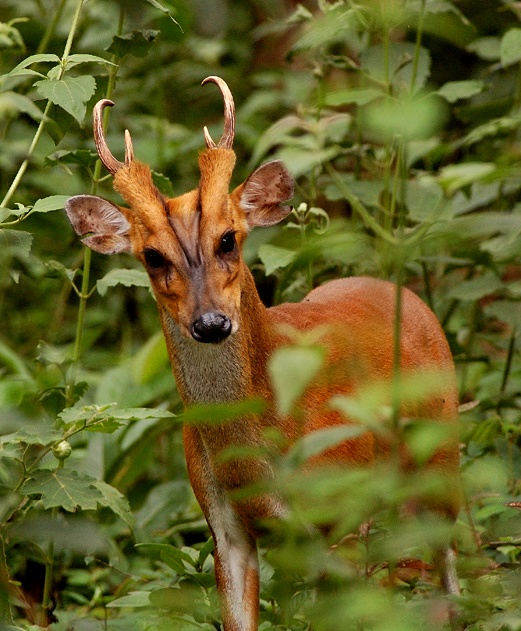
\includegraphics[width=0.7\textwidth]{ch_inference_for_props_oi_biostat/figures/eoce/barking_deer_chisq_gof/barking_deer.jpg} \\
%{\footnotesize photo by shrikant rao (\oiredirect{textbook-flickr_shrikant_rao_barking_deer}{http://flic.kr/p/4xjdkk}) \oiredirect{textbook-cc_by_2}{cc~by~2.0~license}}
\end{center}
\end{minipage}
}{}



